\documentclass[]{article}
\usepackage{graphicx}

%opening
\title{CPSC425 A3}
\author{Eric Semeniuc - 54383161}

\begin{document}

\maketitle
\pagebreak

\textbf{Donkey:}\\
	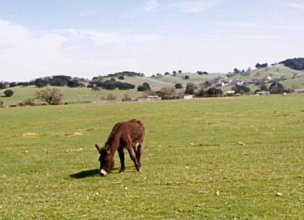
\includegraphics{donkey.jpg}
	\label{fig:donkey}

\textbf{Donkey Result, sd = 1, patchL=10:}\\
	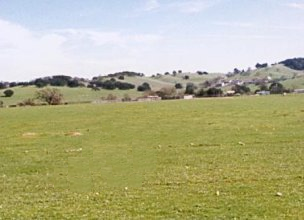
\includegraphics{donkey_results_sd1.jpg}
	\label{fig:donkey_results}

\pagebreak

\textbf{Moto Jump:}\\
	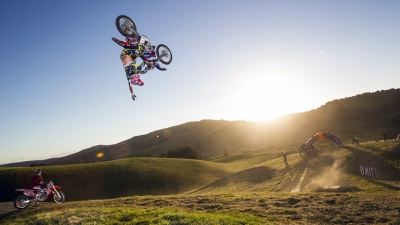
\includegraphics{moto2.jpg}
	\label{fig:moto2}
\textbf{Moto Jump Results, sd = 1, patchL = 2:}\\
	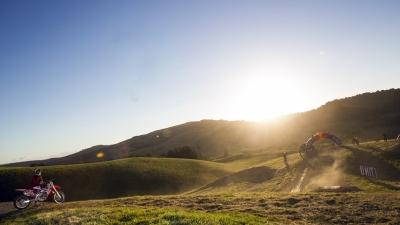
\includegraphics{moto2_results_patch2.jpg}
	\label{fig:moto2_results}
	\textbf{Moto Jump Results, sd = 1, patchL = 10:}\\
	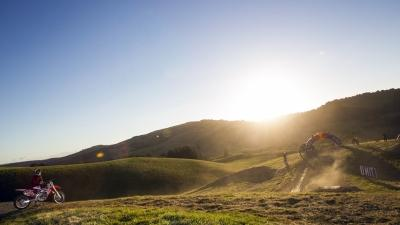
\includegraphics{moto2_results_patch10.jpg}
	\label{fig:moto2_results}
Explanation: The moto jump image works well as the background sky has little noise and a smooth gradient. The image is very predictable and the texture is simple
\pagebreak

\textbf{Box:}\\
	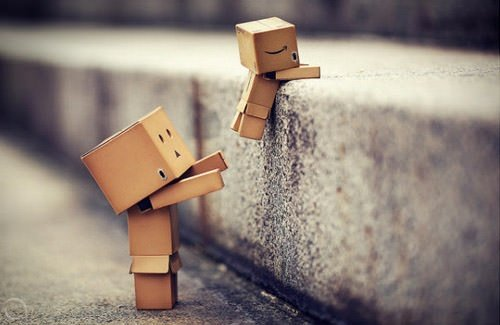
\includegraphics[width=0.7\linewidth]{box.jpg}
	\label{fig:box}\\
\textbf{Box Results, sd = 1, patchL = 10:}\\
	
\includegraphics[width=0.7\linewidth]{box_results.jpg}
	\label{fig:boxresults}\\
The box character image doesn't work well because there is a difference in the smoothness of the image due to the shallow depth of field effect, and the texture is not very consistent with the dirt on the side of the concrete versus the clean top surface of the concrete.


\pagebreak
\textbf{Question 7:}\\
Making randomPatchSD too small creates image artifacts since we can pick up noise rather than the textons\\
Making randomPatchSD too large creates random artifacts as non relevant patches can be selected \\
sd=1\\
	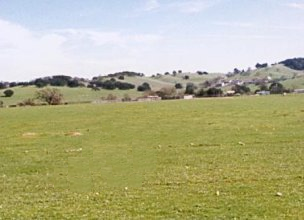
\includegraphics[width=0.7\linewidth]{donkey_results_sd1.jpg}\\
sd=5\\
	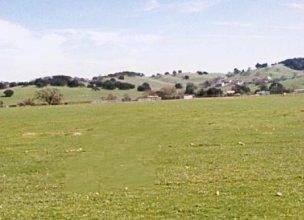
\includegraphics[width=0.7\linewidth]{donkey_results_sd5.jpg}\\
sd=15\\
	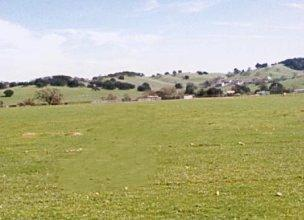
\includegraphics[width=0.7\linewidth]{donkey_results_sd15.jpg}\\
\pagebreak

Making patchL too small can create unwanted patterns (like moire) as we might capture the textons, but not the overall structure of the texture\\
Making patchL too large creates blocky artifacts subsets as we may not have enough samples to choose from for a given patch \\
patchL=2\\
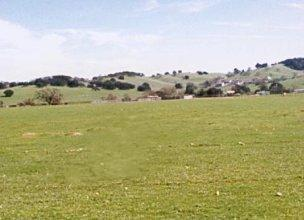
\includegraphics[width=0.7\linewidth]{donkey_results_patch2.jpg}\\
patchL=10\\
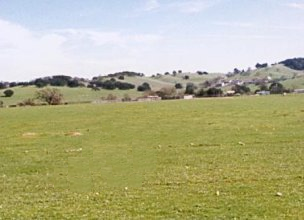
\includegraphics[width=0.7\linewidth]{donkey_results_sd1.jpg}\\
patchL=20\\
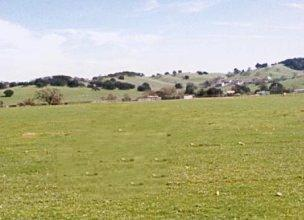
\includegraphics[width=0.7\linewidth]{donkey_results_patch20.jpg}\\



\end{document}
